%\documentclass[aps,prl,twocolumn,showpacs,superscriptaddress,groupedaddress]{revtex4-1}  % for review and submission
%\documentclass[aps,preprint,showpacs,superscriptaddress,groupedaddress]{revtex4-1}  % for double-spaced preprint

%Phys Rev B
%Letter or rapid communication - 3500 words
%\documentclass[prb,groupedaddress,reprint]{revtex4-1}
%APL
\documentclass[aps,prl,twocolumn,showpacs,superscriptaddress,groupedaddress]{revtex4-1}
%\documentclass[aps,prl,reprint]{revtex4-1}
%\documentclass[aip,jap,reprint]{revtex4-1}
\usepackage[english]{babel}
\usepackage{graphicx}% Include figure files
\usepackage[pdftex,unicode,colorlinks, citecolor=blue,%
filecolor=black, linkcolor=blue, urlcolor=black]{hyperref}
\usepackage[figure,table]{hypcap} %links should lead to the begining
                                %of figure or table...

\begin{document} %Max size in pdf for APL - 4 print pages

\title{Super absorption and efficient absorption of light by spherical
  nanoparticles}


\author{Konstantin Ladutenko} \email[e-mail: ]{fisik2000@mail.ru}
\affiliation{ITMO University, 49 Kronverskii Ave., St.~Petersburg
  197101, Russian Federation\\}

\affiliation{Ioffe Physical-Technical Institute of the Russian Academy
  of Sciences, 26 Polytekhnicheskaya Str., St.~Petersburg 194021,
  Russian Federation}

\author{Ovidio Pe\~{n}a-Rodr\'{i}guez} \affiliation{Instituto de
  Fusi\'{o}n Nuclear, Universidad Polit\'{e}cnica de Madrid,\\
  Jos\'{e} Guti\'{e}rrez Abascal 2, E-28006 Madrid, Spain}


% \author{Irina Melchakova} \author{Alexander Shalin}
% \affiliation{ITMO University, 49 Kronverskii Ave., St.~Petersburg
% 197101, Russian Federation\\} TODO не хватает адреса
% \affiliation{Kotel’nikov Institute of Radio Engineering and
% Electronics of RAS (Ulyanovsk branch),\\48 Goncharov Str., Ulyanovsk
% 432011, Russian Federation} \affiliation{Ulyanovsk State University,
% 42 L. Tolstoy Str., Ulyanovsk 432017, Russian Federation}
% \author{Ilya Yagupov} \author{Pavel Belov} \affiliation{ITMO
% University, 49 Kronverskii Ave., St.~Petersburg 197101, Russian
% Federation\\}
\author{Ali Mirzaei} \author{Andrey Miroshnichenko} \author{Ilya
  Shadrivov} \affiliation{Nonlinear Physics Centre, Research School of
  Physics and Engineering, The Australian National University, 59
  Mills Rd, Acton, ACT, 2601, Australia}

\date{\today}
% APL 250 words! Moreover, some designs have spectral Phys Rev B less
% then 500 words, about 5% ot total paper length
% emacs M-x count-words

\begin{abstract}
  Spherical subwavelength nanoparticles have a fundamental limit as to
  how much light they can absorb. This limit is based on the
  assumption that only one mode is excited in the nanoparticle. Using
  genetic algorithm, we design multi-layer nanoparticles, in which we
  can make several resonant modes overlap at the same frequency, thus
  significantly beating the theoretical limit of absorption, and we
  call this super-absorption. We further introduce the efficiency of
  the absorption for a nanoparticle, which is absorption normalized by
  the physical size of the particle, and show that efficient absorbers
  are not always operating in super-absorbing regime.
\end{abstract}


\pacs% insert suggested PACS numbers in braces on next line
{41.20.Jb 42.25.Bs 02.60.Pn 02.70.-c}
% 41.20.Jb Electromagnetic wave propagation 42.25.Bs Wave propagation,
% transmission and absorption
%% 42.25.Fx Diffraction and scattering
% 02.60.Pn Numerical optimization 02.70.-c Computational techniques;
% simulations

\maketitle %\maketitle must follow title, authors, abstract and \pacs

Mie theory~[TODO], which is over 100 years old now, describes
interaction of electromagnetic waves with spherical particles. Mie
solution is still of great interest these days~[TODO], since it is one
of the primary tools for analyzing wave scattering by spherical
objects. Further development of the Mie theory~\cite{Yang-2003,
  Pena-scattnlay-2009} made it possible to apply study the
multilayered spherical particles [TODO]. Such particles have various
applications in cancer treatment [TODO 5,6 from Ovidio draft] and
medical diagnostics [TODO 7 from Ovidio draft],
cloaking~\cite{Semouchkina-2013, Ladutenko-2014} and plasmonic~[TODO]
devices, as well as for improving solar cells performance [TODO].

The scattering properties of multilayer cylinders and spheres was
studied in great detail by Fan~et~al.~[Fan-PRL, Fan-APL]. In these
works authors introduced the concept of a super scattering, when the
scattering cross-section of a multilayer particle exceeds that of a
homogeneous particle of the same size in the so-called single-channel
limit. The super scattering appears when we design a multilayer
structure so that several modes become nearly degenerate, i.e. their
resonance frequencies coincide or get close to each other. In a
homogeneous particle, the resonances appear at different frequencies,
and there is no design freedom for a fixed geometry of the structure
to make these resonances overlap, and this limits the achievable
scattering cross-section.

Similar fundamental limitations exist for the absorbing properties of
sub-wavelength nanoparticles.  Tribelsky [TODO] has derived a
theoretical limit of a maximum absorption cross-section (ACS) value
for a single channel, i.e., when only one mode of the sphere is
excited.  As a result the absorption coefficients $\tilde{a}_n= {\rm
  Re}\{a_n\} - |a_n|^2 $ and $\tilde{b}_n= {\rm Re}\{b_n\} - |b_n|^2 $
become limited by $1/4$, here $a_n$ and $b_n$ are scattering
coefficient as defined in Mie theory [TODO Bohren Huffman]).

To overcome these limitations, we employ similar approach for
enhancing absorption cross-section [Fan-APL]. In particular, we
propose to use the multi-layer structures, and by means of genetic
algorithm we optimize the ACS of these particles. We analyze the
absorption cross-section of these particles, and present the
super-absorption regime. We further introduce the absorption
efficiency, which is the ACS normalized to the geometric cross-section
of the particles. Here we show that there is a strong counter-play
between the increased absorption for larger particles vs size for
smaller particles, and quite remarkably we find that the most {\em
  efficient} absorption can be achieved in a single channel limit for
small particles.

We start our analyses by considering the triple layered $Si/Ag/Si$
spherical particle illuminated with a plane wave~(Fig. TODO ). In what
follows we describe the materials using experimentally measured
parameters from the Ref.~[TODO].  To optimize the thickness of each
layer we implemented~[link to GitHub] an adaptive differential
evolution algorithm~\cite{Storn-DE-first-1997}, which is called
JADE~\cite{Jingqiao-JADE-2009}.  The technical details of the
optimization algorithm are published previously in
Ref.~\cite{Ladutenko-2014}. We perform Mie calculations using the
Scattnlay~\cite{Pena-scattnlay-2009} software, whose results were
verified with a number of other implementations of the Mie solutions
and with a commercially available software such as CST Microwave
studio.

It is obvious that in general, a bigger particle will have a bigger
absorption cross-section, so sphere with the diameter of 1 cm will
absorb more light than any sphere at the nanoscale. Therefore, we use
absorption efficiency $Q_{\rm abs}=C_{\rm abs}/2\pi R_{\rm total}^2$,
where $R_{\rm total}$ is the outer radius of the particle and $C_{\rm
  abs}$ is the absorption cross-section. We maximize absorption
efficiency at a fixed wavelength of incident light (we have chosen
$\lambda=500$~nm).

\begin{figure}
  \center{
    % Use pdfcrop to remove white margins
    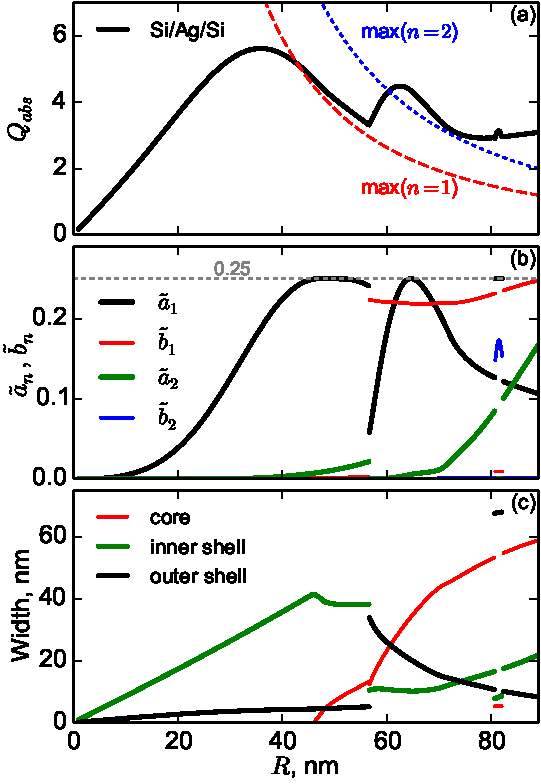
\includegraphics[width=0.4\textwidth]{fig/2015-04-01-Qabs-SiAgSi-overview}%
    \caption{ Results of the optimization of the absorption efficiency
      for the fixed wavelength of 500~nm. (a) Absorption efficiency
      with the best value achieved at the particle radius of 36~nm and
      Ag/Si design (zero sized core). Dashed lines show theoretical
      limits for the first channel and second channel
      absorption. Second and third peaks in the absorption efficiency
      curve exceed the theoretical limit for the second mode
      absorption at R=63~nm and R=81~nm. (b) Mie
coefficients for individual excited modes of the optimized structures
[Kostya - why do they have tildas - are these not directly Mie
coefficients?]. (c) Optimized layer thicknesses. For the total
particle radius below 46~nm the genetic algorithm converges to the
two-layer structure, when core size vanishes, and the optimum design
is a bi-layer $Ag/Si$ particle. 

      \label{fig:overview}
    }%
  }
\end{figure}
%
In order to study the dependence of the absorption efficiency on the
outer particle size, we run optimization algorithm for different
(fixed) particle outer size, and our optimization parameters are the
radii of internal cores, whereas the target function is the absorption
efficiency.  We show the results of our genetic optimization algorithm
in Fig.~\ref{fig:overview}a.  Dashed lines show theoretical absorption
limit of a dipole ($n=1$) and a quadrupole ($n=2$)
resonances~[Tribelsky:TODO], which are given as $$Q^{(n)}_{\rm abs\
  max}=\frac{2n+1}{2q^2},$$ where the size parameter $q=2\pi R_{\rm
  total}/\lambda$, and $n$ is an angular momentum of the
mode. Following Ref.~[Fan-APL], where authors introduce super
scattering for spherical particles, here we we introduce
super-absorption, when the ACS is larger than the theoretical limit
for absorption by the mode with highest excited angular momentum
$n$. In our parameter space we have just modes up to the quadrupole
excited ($n=2$), and in order to get a super-absorption our efficiency
should be higher than that of a quadrupole. We clearly see this
super-absorption at $R_{\rm total}>60$~nm, in Fig.~\ref{fig:overview}
(a).

In Fig.~\ref{fig:overview}b we present the values of Mie coefficients
for individual excited modes in the structure, while horizontal dashed
line shows the theoretical limit (1/4) for each of
them. $\tilde{a}_{1,2}$ are electric dipole and electric quadrupole,
while $\tilde{b}_{1,2}$ are magnetic dipole and magnetic
quadrupole. For small particles, as expected, the absorption is
dominated by an electric dipole $\tilde{a}_1$.  At $R_{\rm total} >
56.6$~nm the optimization procedure finds that the designs with both
electric and magnetic dipoles have larger ACS, than the structure with
only the electric dipole excited. This is why the curves in
Figs.~\ref{fig:overview} (b,c) experience the discontinuity. We also
note that there is a very narrow range of particle sizes, between
80.7~nm and 82.1~nm, where our analyses finds that the design
supporting electric dipole $\tilde{a}_1$ and magnetic quadrupole
$\tilde{b}_2$, has larger ACS, and this explains two more
discontinuities of the curves at the respective size values.

Fig.~\ref{fig:overview} (c) shows optimized sizes of the layers inside
the multi-layer structure. It reveals quite a curious result, that the
dipole branch (i.e. for particle radii below 56.6~nm) has two
parts. For $R_{\rm total}<46$~nm the best absorber has just two
layers, as the radius of the core of the three-layer structure
vanishes, and the particle reduces to $Ag/Si$ core-shell structure.
At $R_{\rm total}=46$ dipole channel becomes practically
undistinguishable from the theoretical limit (it becomes
$\tilde{a}_1>0.249$).  It appears that the optimizer introduced the
inner $Si$ layer in order to keep $\tilde{a}_1$ near the theoretical
limit as the $R_{\rm total}$ increases.  As a side effect, the
quadrupole contribution $\tilde{a}_2$ appears, however, it does not
help to reach super-absorption limit $n=2$.

Remarkably, the absolute maximum absorption efficiency is not reached
within the super-absorption regime. Figure~\ref{fig:overview} shows
that the maximum efficiency is reached for small particle size, and
the ACS is still well below the single channel limit. It appears that
the $Ag/Si$ core-shell nanoparticle, with the total radii of
approximately 36~nm is the most efficient absorbing in the considered
structure, which ACS reaching values over 5 times the physical
cross-section area of the particle.  From practical point of view it
is quite important that the maximum can be reached in a bi-layer
structure, instead of a triple-layer, and it should be easier and
cheaper to produce.

\begin{figure}
  \center{
    % Use pdfcrop to remove white margins
    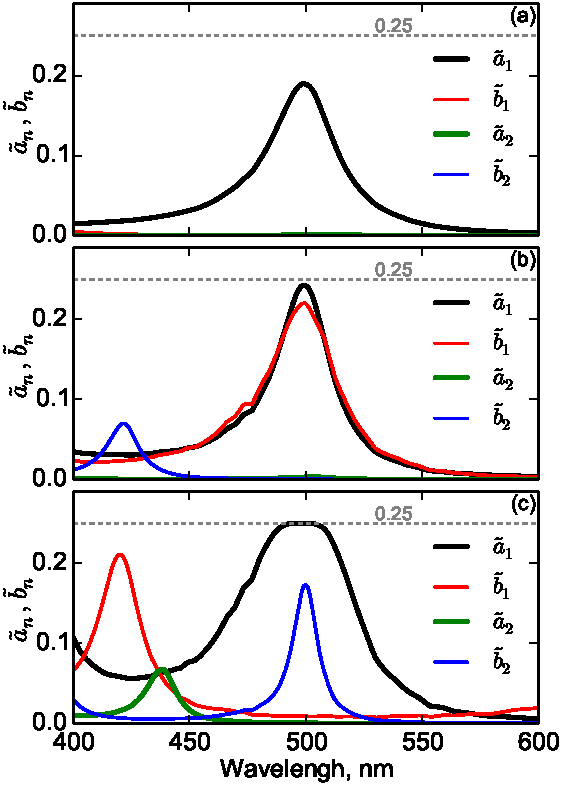
\includegraphics[width=0.4\textwidth]{fig/2015-04-01-SiAgSi-ab-spectra3.pdf}%
    \caption{Spectra of Mie coefficients of (a) efficient and (b-c)super absorption design.      
      \label{fig:spectra}
    }%
  }
\end{figure}
%
To study spectral properties of the structures with large ACS which we
obtained by the optimization, in Fig.~\ref{fig:spectra} we plot three
different cases for designs that correspond to local maxima of $Q_{\rm
  abs}$ shown in Fig.~\ref{fig:overview} (a).  As expected, the design
corresponding to the maximum absorption efficiency at R=36~nm has a
single electric dipole resonance centered at the target wavelength
$\lambda=500$~nm. Spectra of designs with maxima at R=63~nm and
R=81~nm have a signature of the super absorption, i.e. there is an
overlap of several resonances.  We note that these structures have
additional absorption resonances, but they are located far from the
wavelength of interest.  A noticeable feature of
Fig.~\ref{fig:spectra} (c) is an almost flat top of the electric
dipole resonance. (TODO add some explanation, why it flat? Any ideas?
- not really, maybe there are two different dipole "types", and we see
their interference?)

\begin{figure}
  \center{
    % Use pdfcrop to remove white margins
    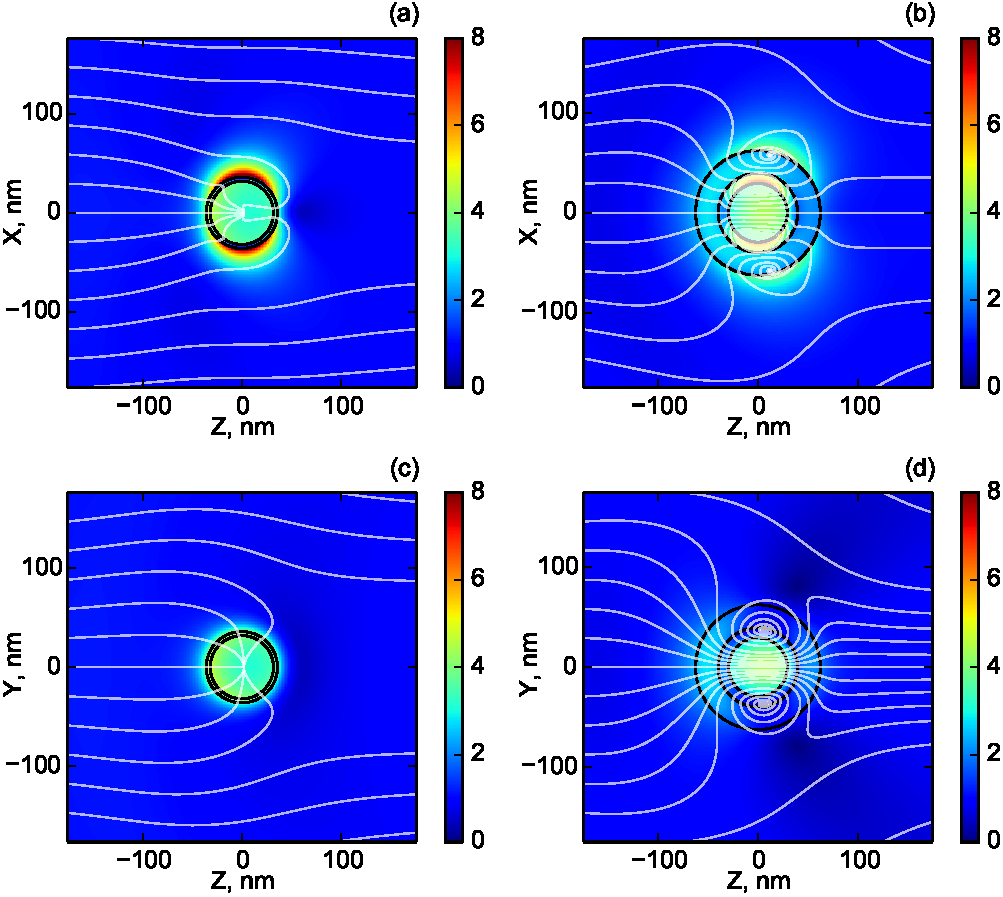
\includegraphics[width=0.4\textwidth]{fig/SiAgSi-flow-R62-YZ-Eabs.pdf}%
    \caption{ Amplitude of electric field for R=36 nm (a,c) and
      ``super'' (b,d) designs in E-k  (a-b) and H-k (c-d) planes. 
      \label{fig:field}
    }%
  }
\end{figure}
%
Finally, we present distribution of the amplitude of the electric
field in Fig.~\ref{fig:field} for two designs: with the best
efficiency at R=36 nm and in a super-absorbing design with R=???? nm.
We set different scale for these two designs so that black circles
that denote outer boundary are plotted to be the same size [I am
actually not convinced that this is the best way to present it. Can
you show them in "true" scale?].  We also plot streamlines of the
Poynting vector which characterize energy flow. For the effective
design of the absorber, the power from a large cross-sectional area
flows into the particle.  In case of super-absorption regime, we
observe power flow vortices, which make absorbtion more efficient as
the electromagnetic energy propagates several times through the
absorbing materials.




% . Our initial idea was to show the same effect in absorption, and
% R=63 with R=81nm are such `superabsopting` designs. However, in 3D
% case (in contrast to 2D investigated with Ali) it turned out that
% sometimes it is preferable to use a smaller particle with single
% resonance to achieve the best efficiency. This way, in 3D case using
% real materials for a multilayer spherical particle
% ``superabsorbing'' design do not always leads to best absorption
% efficiency. Moreover, same effect exists for scattering from SiAgSi
% optimized structure. At WL=500 nm ``super'' scattering mode with two
% resonances gives the best efficiency, however, at WL=400 nm a single
% resonance small particle has a better scattering efficiency compared
% to larger particles with ``super'' design.







% \begin{acknowledgments}
%   The authors would like to thank the Ministry of Education and
%   Science of the Russian Federation (Goszadanie 2014/190, Zadanie
%   No. 3.561.2014/K, project 14.584.21.0009 10), Russian Foundation
%   for Basic Research (Grant 15-02-01344), and Government of the
%   Russian Federation (Grant 074-U01) for the financial support. The
%   simulations of cloak designs has been funded by the Russian
%   Science Foundation Grant No. 14-12-01227.% We
%   %   would also like to appreciate Alexander Krasnok for the help
%   %   with
%   %   CST simulations and Ilya V. Shadrivov for valuable comments on
%   %   the
%   %   manuscript.
% \end{acknowledgments}

In conclusion, we find the effect of the super-absorption, when the
absorption cross-section of the nanoparticle can exceed the
theoretical limit for the absorption by the highest excited mode. This
occur when several resonance modes of the structure overlap at the
same frequency. We introduce efficiency of the absorption as an
absorption cross-section divided by a geometric cross-section of the
particle, and quite unexpectedly we find that the most efficient
absorbers are smaller nanoparticles working in a single mode
regime. We present their spectral characteristics and field structure.


WE NEED TO WRITE ABOUT THIS AND SOME OTHER WORKS IN THE
INTRODUCTION. THE TOPIC IS DONE TO DEATH. It is intersting, that
similar conclusion was made by Miller et al~[TODO Fundamental Limits
to Extinction by Metallic Nanoparticles Phys. Rev. Lett. 112, 123903 –
Published 26 March 2014 O. D. Miller, C. W. Hsu, M. T. H. Reid,
W. Qiu, B. G. DeLacy, J. D. Joannopoulos, M. Soljačić, and
S. G. Johnson] for extinction of arbitrary particles.


\bibliography{2015-Ladutenko-Qabs}
\end{document}

